\section{Guia de Instalação}

\begin{frame}{Guia de Instalação}{}
\begin{block}{Instalação da Ferramenta}
  \begin{itemize}
    \item<1-> sudo apt-get install subversion libapache2-svn
  \end{itemize}
\end{block}
\end{frame}
%%%%%%%%%%%%%%%%

\begin{frame}{Guia de Instalação}
\begin{block}{Vasta documentação para o processo de instalação}
  \begin{itemize}
    \item<1-> Diversos SO's
    \item<1-> Diversos maneiras
  \end{itemize}
\end{block}
\end{frame}
%%%%%%%%%%%%%%%%

\begin{frame}{Guia de Instalação}
\begin{block}{Dificuldade para a instalação por meio do código fonte}
  \begin{itemize}
    \item<1-> Dependência de outras bibliotecas auxiliares
  \end{itemize}
\end{block}
\end{frame}
%%%%%%%%%%%%%%%%

\begin{frame}{Guia de Instalação}
\begin{block}{Dificuldade para a instalação por meio do código fonte}
  \begin{figure}[h!]
    \centering
      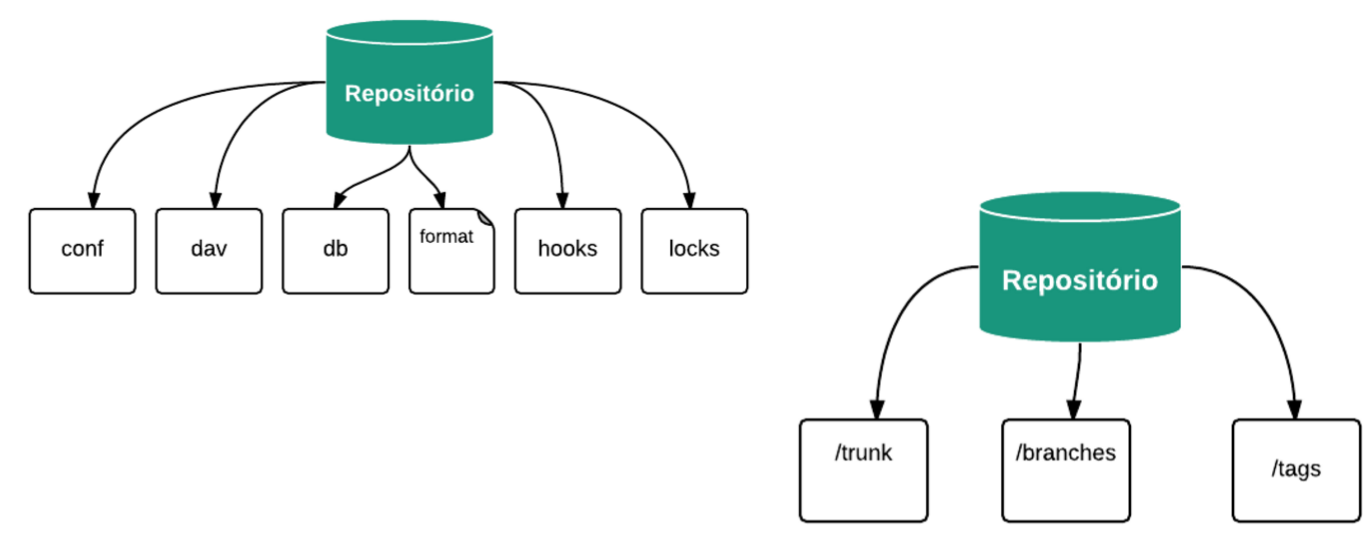
\includegraphics[width=1\textwidth]{figuras/repo}
  \end{figure}
\end{block}
\end{frame}
%%%%%%%%%%%%%%%%

\begin{frame}{Guia de Instalação}
\begin{block}{Cópia de trabalho}
  \begin{figure}[h!]
    \centering
      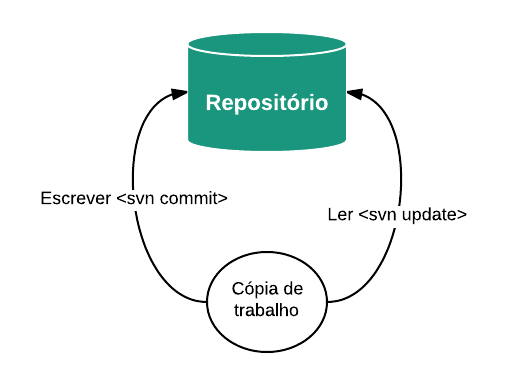
\includegraphics[width=1\textwidth]{figuras/repositorio_copia}
  \end{figure}
\end{block}
\end{frame}
%%%%%%%%%%%%%%%%
